\begin{center}
\textsc{\Large Laboratorio 7}~\\
{\large Vídeo Juegos, Programación, Diseño}~\\
\emph{Event Logging y Manejo de Usuarios}
\end{center}

\section{Pre-Laboratorio}
\begin{itemize}
\item Investigar los siguientes conceptos:
\begin{enumerate}
  \item Software tracing, event logging y sus diferencias.
  \item Software Multi-usuario
\end{enumerate}
\item De algún juego que conozca analice.
\begin{enumerate}
  \item ¿En alguna forma este juego guarda información de su progreso?
  \item Si la pregunta 1. es positiva, ¿de que forma es utilizada esta información?
\end{enumerate}
\item Investigue o nombre algún juego que conozca que permita el manejo de varios usuarios. ¿De que forma el juego maneja multiples usuarios?
\end{itemize}

\section{Event Logging}
Los vídeo juegos actuales son piezas de software de gran complejidad por lo tanto mantener un historial de información durante la ejecución del programa puede ser de inmensa ayuda para distintos propósitos. Esta información es usualmente utilizada para debugging pero dependiendo del tipo de información guardada esta puede ser usada para una gran cantidad de propósitos \cite{colm_tracing}.
\newpage
\setlength\intextsep{0pt}
\begin{wrapfigure}[11]{r}{0.3\linewidth}
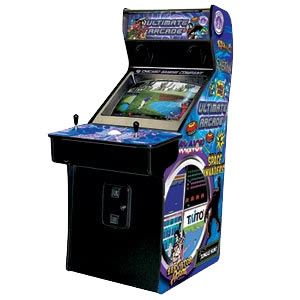
\includegraphics[width=\linewidth]{semana7/arcade-machines.jpg}
\caption{En los arcade juegan multiples usuarios \cite{arcade_score}.}
\label{fig:arcade}
\end{wrapfigure}
\section{Manejo de Usuarios}
Los vídeo juegos usualmente puede ser jugados por mas de un usuario incluso si este vídeo juego es de un solo jugador, con cada usuario teniendo su propia sesión de juego, esta sesión de juego puede guardar cosas tan sencillas como el nombre de usuario para propósitos de personalización o datos mas complejos como actual posición en el transcurso del juego, puntuación, logros, objetivos actuales, etcétera, todo esto dependiente del diseño del juego.

\section{Actividad}
\todo[inline]{Por hacer.}